\section{DRL}   


\begin{frame}{Deep Reinforcement Learning (DRL) Model}
    \tableofcontents[sectionstyle=show/hide, hideothersubsections]
    \centering
    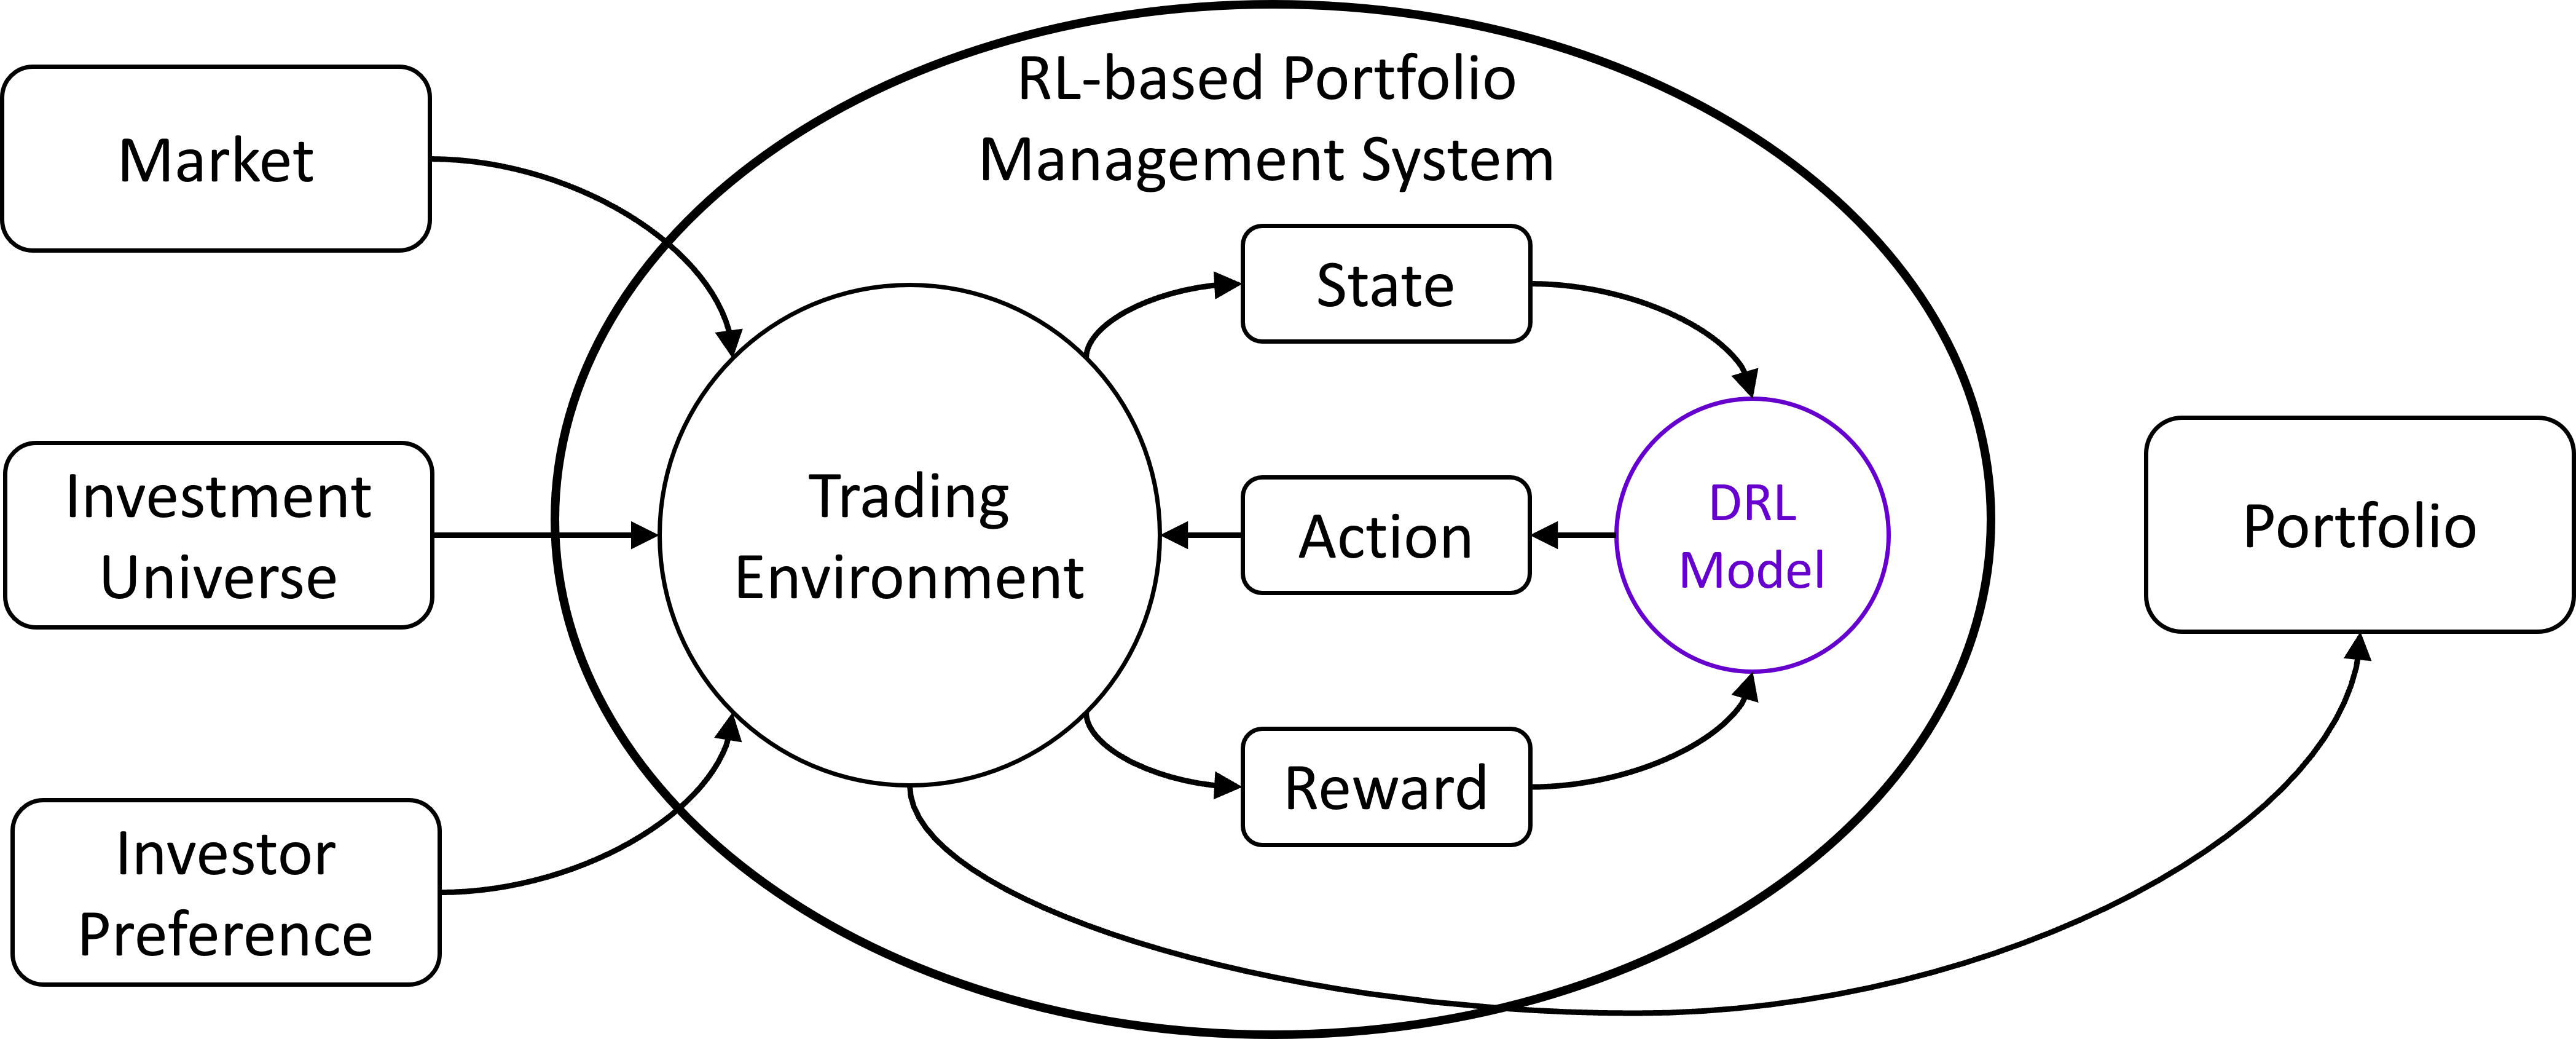
\includegraphics[width=10cm]{images/drl_model.png}
\end{frame}

\subsection{Reinforcement Learning}
\begin{frame}{Reinforcement Learning}
\begin{columns}
    \begin{column}{0.45\textwidth}
    \begin{enumerate}
        \item Observes the states from the environment.
        \item Performs the action on the environment.
        \item Adjust its parameters based on the reward.
    \end{enumerate}
    \end{column}
    \begin{column}{0.45\textwidth}
      \centering
    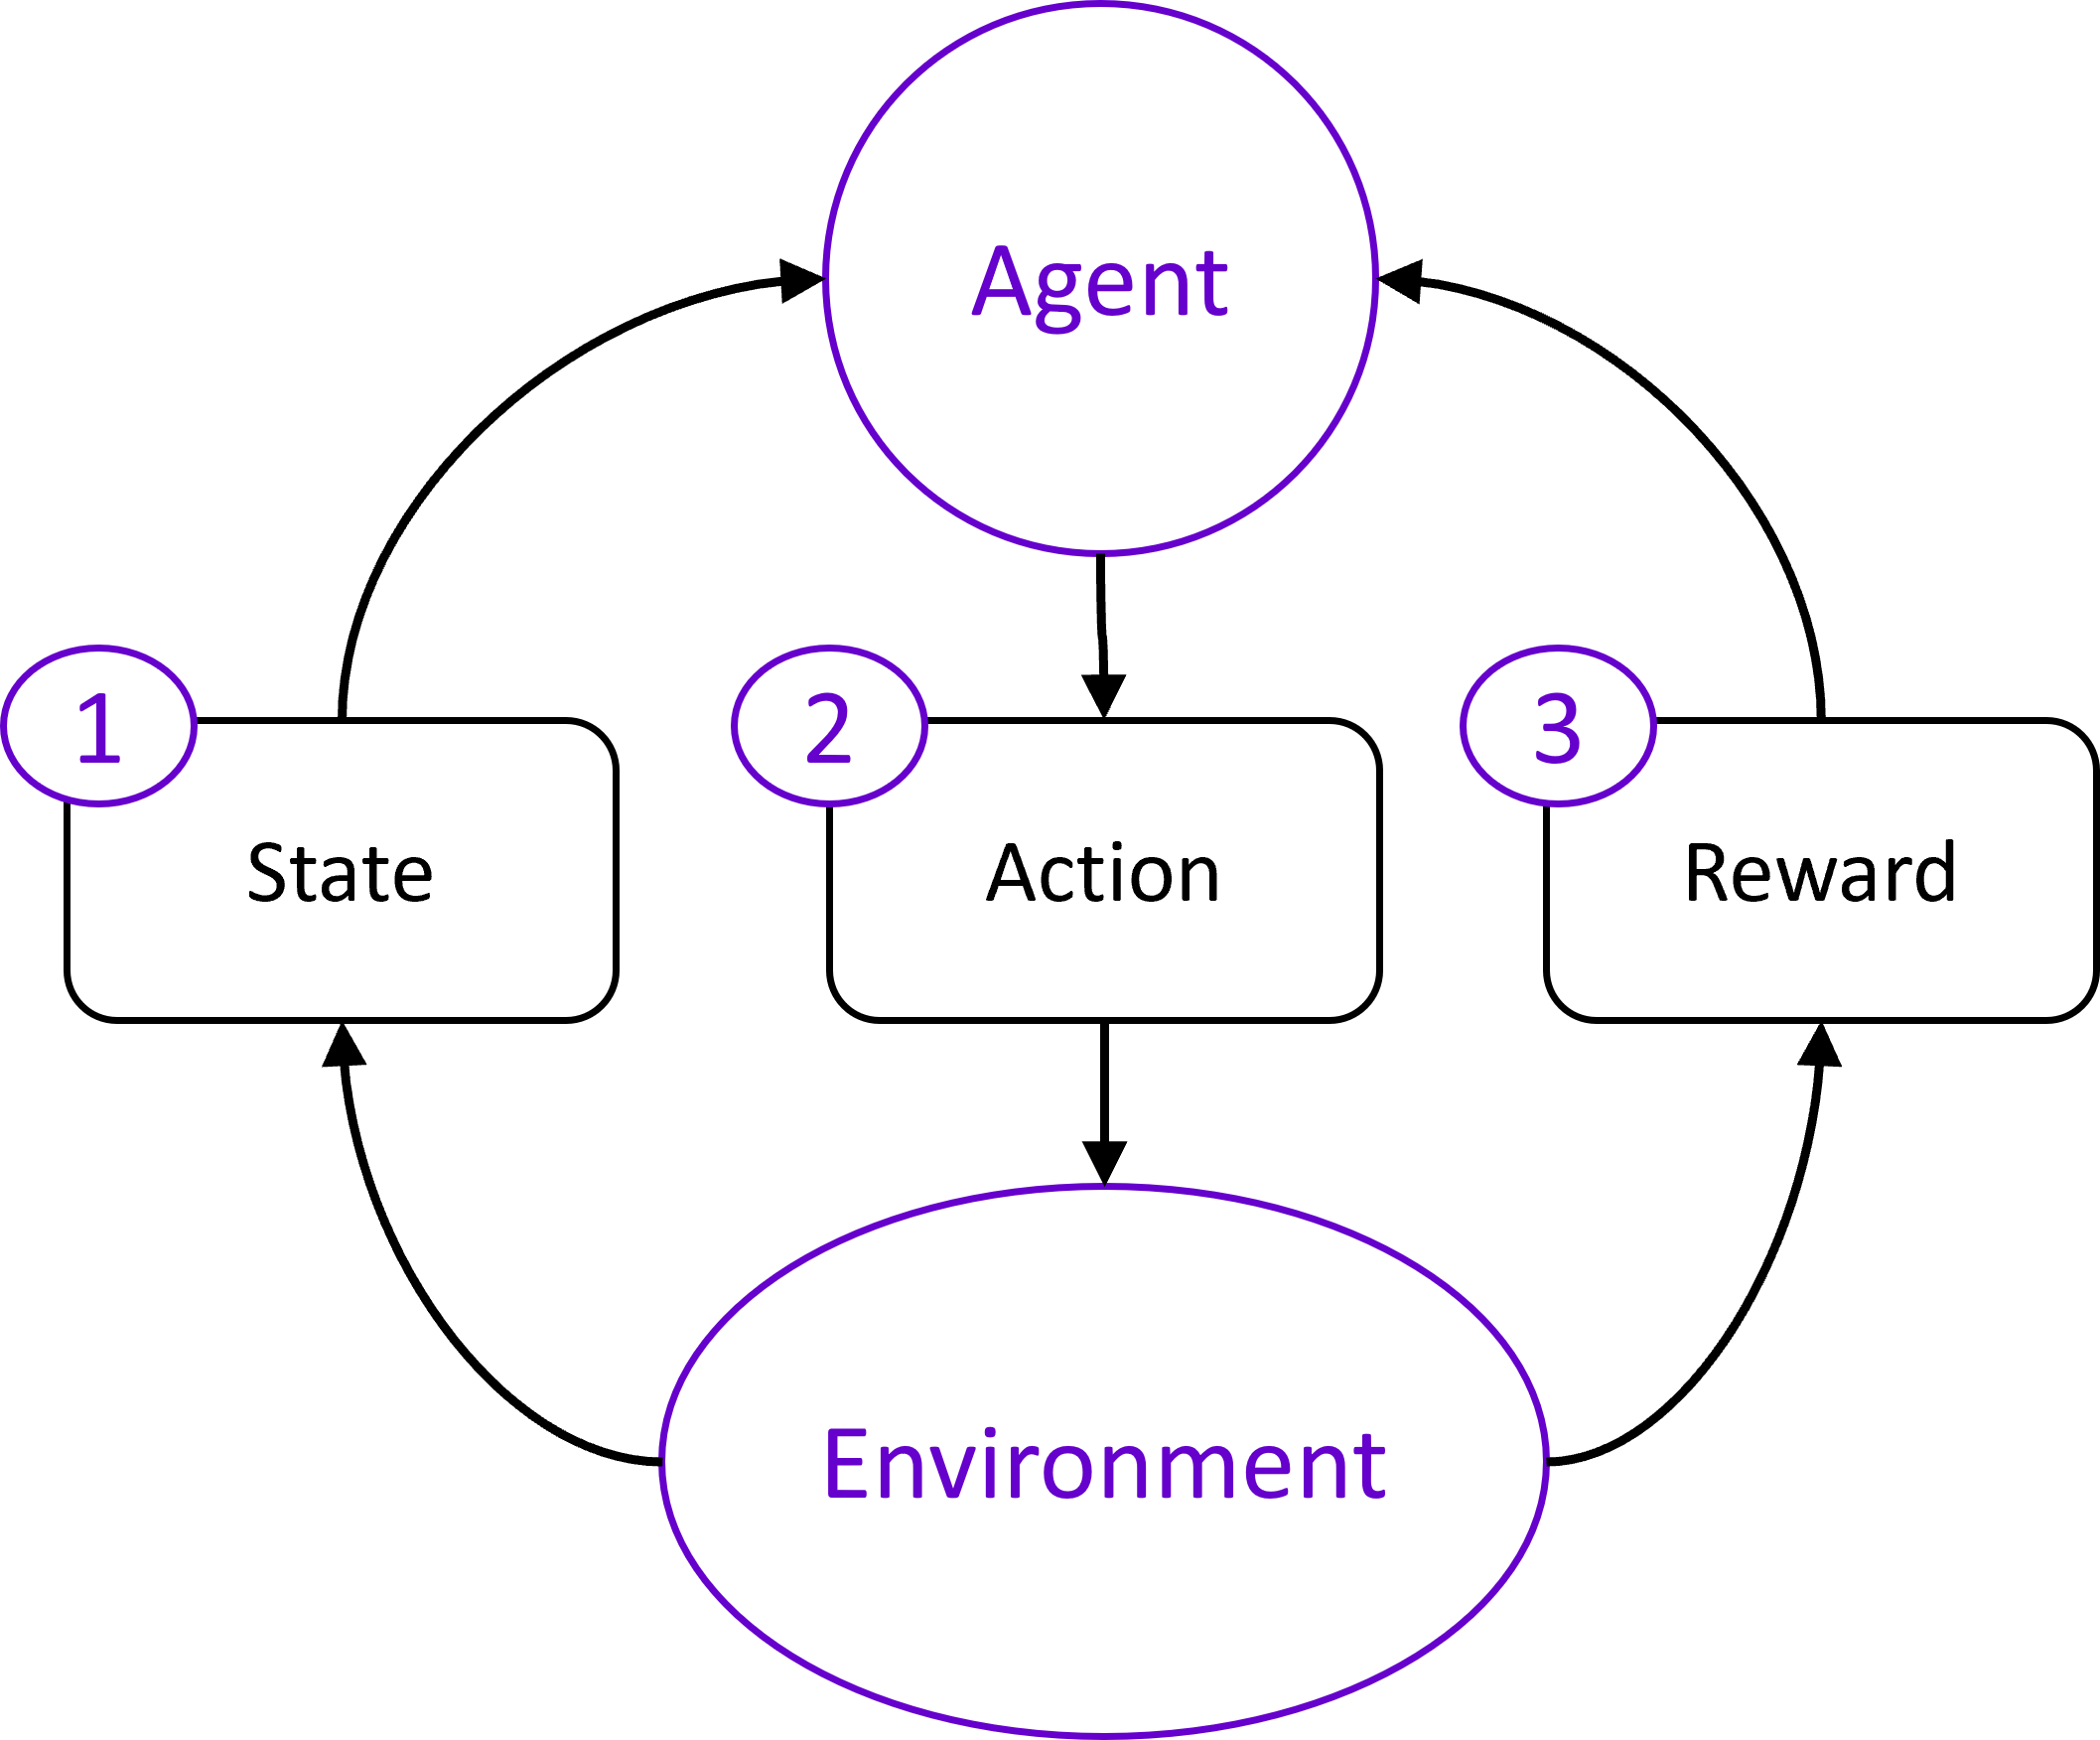
\includegraphics[width=5cm]{images/rl_overview.png} \end{column}
\end{columns}
\end{frame}


\subsection{Value Optimization vs Policy Optimization}
\begin{frame}{Value Optimization vs Policy Optimization}
\begin{block}{Value Optimization}
\begin{itemize}
    \item Optimize the value function (The function estimate the expected reward with given state and action)
    \item \alert {Challenges for continuous action,  the output space will be enormous}
\end{itemize}
\end{block}
\begin{block}{Policy Optimization}
    \begin{itemize}
        \item Optimize the policy (the agent's strategy to perform the action)
        \item \color{blue}{Works well for continuous action}
    \end{itemize}

\end{block}
\end{frame}

\subsection{On-Policy vs Off-Policy}

\begin{frame}{On-Policy vs Off-Policy}
    \begin{block}{On-Policy}
        \begin{itemize}
        \item Behavior Policy =  Target Policy
        \item \alert{Need full episode before optimizing, low sample efficiency}
    \end{itemize}
    \end{block}
        \begin{block}{Off-Policy}
        \begin{itemize}
        \item Behavior Policy $\neq$ Target Policy
        \item \color{blue}{Can update policy afer each step, high sample efficiency with experience replay}
    \end{itemize}
    \end{block}
\end{frame}


\subsection{Determinisitc Policy vs Stochastic Policy}
\begin{frame}{Determinisitc Policy vs Stochastic Policy}
    \begin{block}{Determinisitc Policy}
        \begin{itemize}
        \item Determinisitc actions
        \item \alert{Might trap on local optima due to lack of exploration}
    \end{itemize}
    \end{block}
    
    \begin{block}{Determinisitc Policy}
        \begin{itemize}
        \item Probability distribution over actions
        \item \color{blue}{Avoid trap on local by  exploration}
    \end{itemize}
    \end{block}    
    
\end{frame}

\begin{frame}{Comparison}
    \begin{columns}[c]
    \begin{column}{0.5\textwidth}
    \begin{block}{DQN}
    \begin{itemize}
        \item \alert{Value Optimization}
        \item \color{blue}{Off-Policy}
        \vspace{0.25in}
    \end{itemize}
    \end{block}
    \begin{block}{TRPO/PPO}
        \begin{itemize}
            \item \color{blue}{Policy Optimization}
            \item \alert{On-Policy}
            \item  \color{blue}{Stochastic Policy}
        \end{itemize}
    \end{block}
    \end{column}
    \begin{column}{0.5\textwidth}
    \begin{block}{DDPG/TD3}
        \begin{itemize}
            \item \color{blue}{Policy Optimization}
            \item \color{blue}{Off-Policy}
            \item \alert{Determinisitc Policy}
        \end{itemize}    
    \end{block}
    \begin{block}{SAC}
        \begin{itemize}
            \item \color{blue}{Policy Optimization}
            \item \color{blue}{Off-Policy}
            \item \color{blue}{Stochastic Policy}
        \end{itemize}    
    \end{block}
    \end{column}
    \end{columns}

\end{frame}



\subsection{Soft Actor-Critic}


\begin{frame}{Soft Actor-Critic}
We Use Soft Actor-Critic (SAC), as the DRL model.
\begin{block}{Actor-Critic}
     \begin{columns}
        \begin{column}{0.45\textwidth}
        \begin{enumerate}
            \item Observes the states from the environment.
            \item Performs the action on the environment.
            \item Calculate TD error based on the reward.
            \item Adjust the parameters of Value function and the policy with the TD error.
        \end{enumerate}
        \end{column}
        \begin{column}{0.45\textwidth}
        \centering
        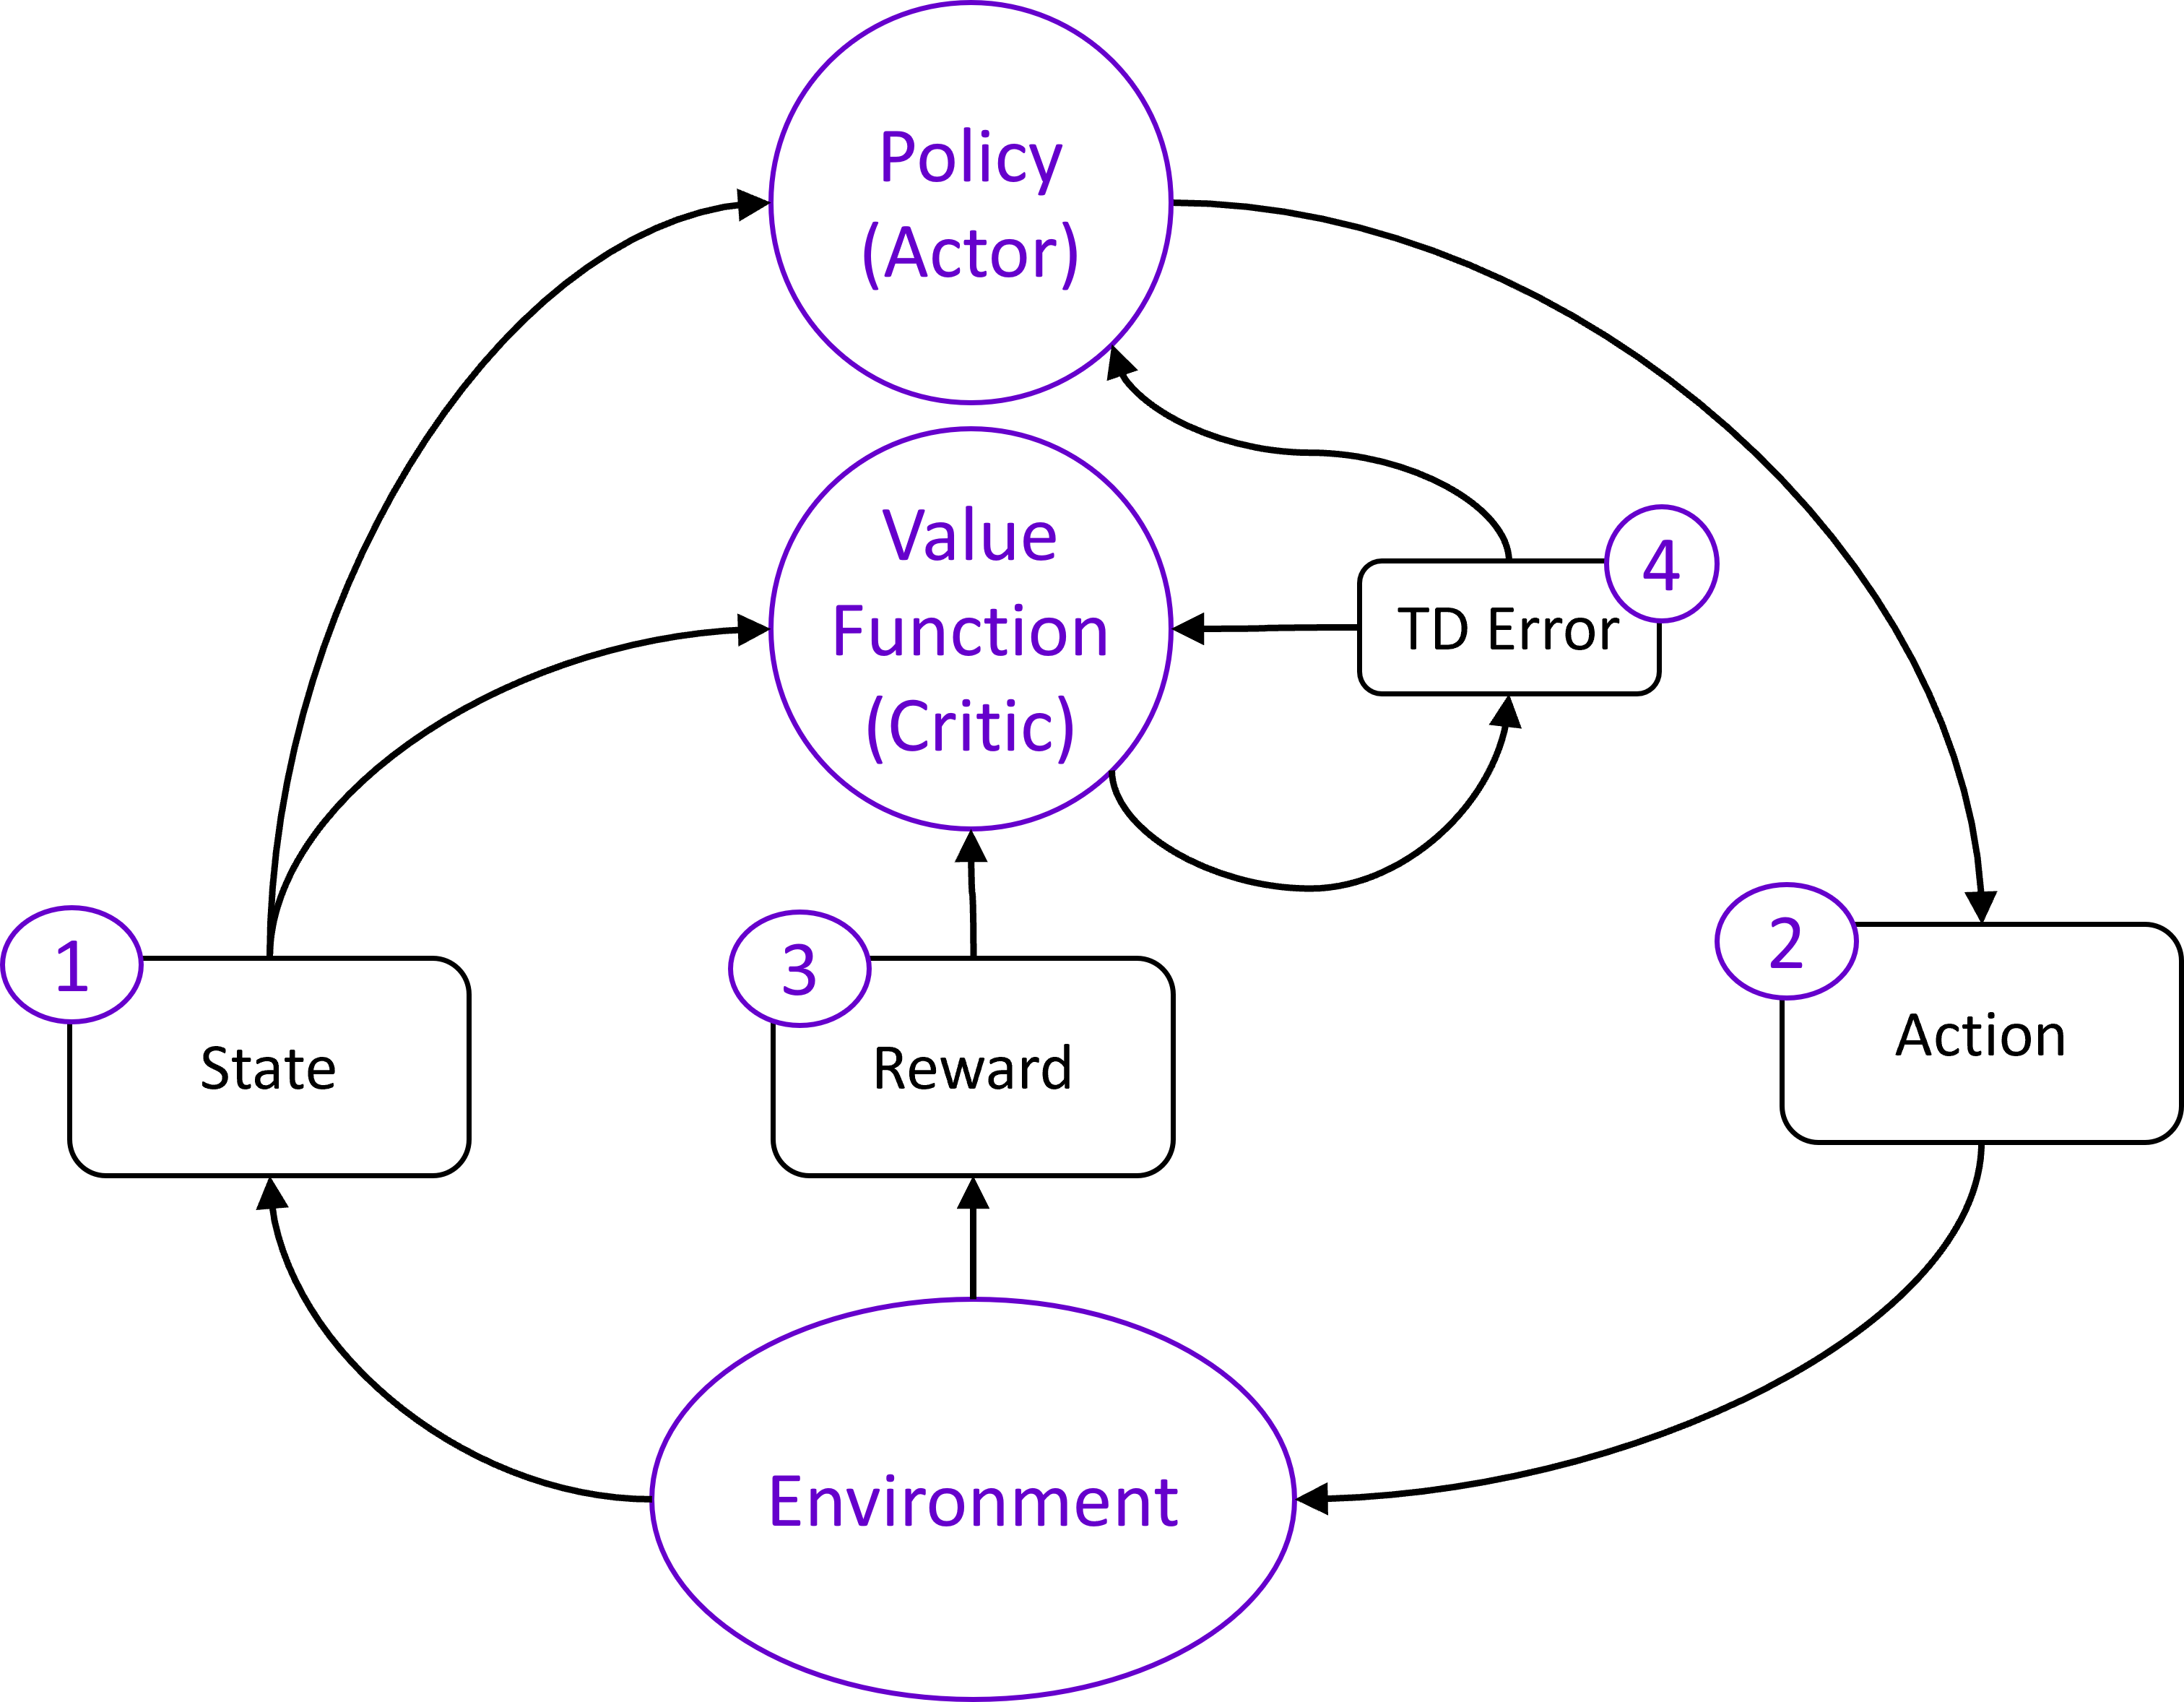
\includegraphics[width=5cm]{images/actor_critic.png}
     \end{column}
     \end{columns}
 \end{block}
\end{frame}

\begin{frame}{Soft Actor-Critic}
We Use Soft Actor-Critic (SAC), as the RL model.
\begin{block}{SAC Overview}
\begin{itemize}
    \item Optimizes a stochastic policy in an off-policy way
    \item Optimizes the policy with \alert{entropy regularization} and takes entropy, measuring randomness in the policy, into account.
\end{itemize}
\end{block}
\begin{alertblock}{Reward Scale}
SAC is highly sensitive to the scaling of the reward. 
\begin{itemize}
    \item Too small, the reward will fail to affect the model, and the policy will become nearly uniform.
    \item Too large, the model will learn quickly and become deterministic, leaving no room for exploration.
\end{itemize}
\end{alertblock}
\end{frame}
